\chapter{Introduction}

The increasing digitization of historical documents has created demand for efficient and accurate methods to categorize and organize these valuable ancient scripts. The field of Deep Learning has met with great success in many problems involving complex data \cite{najafabadi_deep_2015}. The majority of the available digitized corpus is unlabeled and lacks metadata. Consequently, an unsupervised approach to learning is necessary which takes advantage of the large amounts of unlabeled data. Hence, this master project evaluates the efficacy of Deep Learning based Self-supervised Learning approaches in the context of historical documents. Self-supervised learning models extract intrinsic patterns from the data, which is used for knowledge transfer to the target task.

This project focuses on the style classification of Medieval Handwritings in Latin Script and is the target task in this work. Style classification may also be referred to as script type classification in this report. The Script type classification refers to the task of categorizing Latin scripts according to morphological differences in the handwritten text \cite{cloppet_icdar2017_2017}. Representations produced by the self-supervised model are employed to enhance the accuracy of script type prediction by utilizing the morphology present in the text. For this study, it was of interest to investigate \acrfull{simclr} \cite{chen_simple_2020}, \acrfull{mae} \cite{he_masked_2021}, and \acrfull{byol} \cite{grill_bootstrap_2020} \acrfull{ssl} methods. The scope of this project is to compare the quality of generated representations by the mentioned self-supervised learning techniques.

The upcoming chapters of this study will consist of an overview of the dataset and the self-supervised algorithms employed. In addition, the methods utilized will be carefully examined. Subsequently, the results and analysis of the study will be presented.

% % let's show you how \cite and \gls for abbreviations works
% Example paragraph: 

% Useful reads:

% Checkout the subcaption package how to do multiple figures/tables. Make sure
% that you use vector graphics - no blurry png - for graphs or similar, \eg use
% tikz/inkscape. \cref{fig:ex} is an example of a figure using the package tikz. Make also sure that your plots are readable and have axis
% captions, \eg use pgfplots.

% How to create good looking tables with the booktabs package
% e.g. a table should like \cref{tab:ex}.

% \begin{table}
%     \centering
%         \caption[Short title for the List of Tables.]{Long caption for this table which is composed by sub-table 1 and sub-table 2.}
%         \begin{subtable}{.5\textwidth}
%             \centering
%                 \caption{Sub-table 1.}
%             	\begin{tabular}{llr}
%             		\toprule
%             		id & method & result\\
%             		\midrule
%             		1 & A & 0.9\\
%             		2 & B & 0.8\\
%             		\bottomrule
%             	\end{tabular}
%         \end{subtable}% <---- don't forget this %
%         \begin{subtable}{.5\textwidth}
%             \centering
%                 \caption{Sub-table 2.}
%             	\begin{tabular}{llr}
%             		\toprule
%             		id & method & result\\
%             		\midrule
%             		1 & C & 90\%\\
%             		2 & D & 80\%\\
%             		\bottomrule
%             	\end{tabular}
%         \end{subtable}
% \label{tab:ex}
% \end{table}


% \begin{figure}
% \centering
%  \centering
 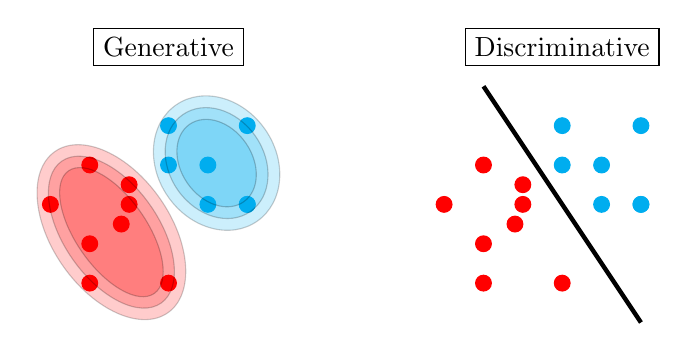
\begin{tikzpicture}[scale=0.5]
  \node[draw] at (3,7) {Generative};

  \draw[draw=red,fill=red] (1,1) circle (0.2);
  \draw[draw=red,fill=red] ( 2 , 3.5 ) circle (0.2);
  \draw[draw=red,fill=red] ( 0 , 3 ) circle (0.2);
  \draw[draw=red,fill=red] ( 1 , 2 ) circle (0.2);
  \draw[draw=red,fill=red] ( 2 , 3 ) circle (0.2);
  \draw[draw=red,fill=red] ( 3 , 1 ) circle (0.2);
  \draw[draw=red,fill=red] ( 1 , 4 ) circle (0.2);
  \draw[draw=red,fill=red] (1.8,2.5) circle (0.2);
  %
  \draw[rotate around={35:(2,2)},fill=red, opacity=0.2] (1.8,2.5) ellipse (1.5 and 2.5);
  \draw[rotate around={35:(2,2)},fill=red, opacity=0.21] (1.8,2.5) ellipse (1.2 and 2.2);
  \draw[rotate around={35:(2,2)},fill=red, opacity=0.22] (1.8,2.5) ellipse (0.9 and 1.9);
  %%%%%%%%%%%%%%%%%%%%%
  \draw[draw=cyan,fill=cyan] ( 4 , 3 ) circle (0.2);
  \draw[draw=cyan,fill=cyan] ( 4 , 4 ) circle (0.2);
  \draw[draw=cyan,fill=cyan] ( 5 , 5 ) circle (0.2);
  \draw[draw=cyan,fill=cyan] ( 5 , 3 ) circle (0.2);
  \draw[draw=cyan,fill=cyan] ( 3 , 4 ) circle (0.2);
  \draw[draw=cyan,fill=cyan] ( 3 , 5 ) circle (0.2);
  \draw[draw=cyan,fill=cyan] ( 5 , 3 ) circle (0.2);
  \draw[rotate around={35:(4.5,4)},fill=cyan, opacity=0.2] (4.3,4.2) ellipse (1.5 and 1.8);
  \draw[rotate around={35:(4.5,4)},fill=cyan, opacity=0.21] (4.3,4.2) ellipse (1.2 and 1.5);
  \draw[rotate around={35:(4.5,4)},fill=cyan, opacity=0.22] (4.3,4.2) ellipse (0.9 and 1.2);
  %%%%%%%%%%%%%%%%%%%%%%%%%%%%%%%%%%%%%%%%%
  \node[draw] at (13,7) {Discriminative};
  \draw[ultra thick] (15,0) -- (11,6cm);
  \draw[draw=red,fill=red] ( 11 , 1 ) circle (0.2);
  \draw[draw=red,fill=red] ( 12, 3.5) circle (0.2);
  \draw[draw=red,fill=red] ( 10 , 3 ) circle (0.2);
  \draw[draw=red,fill=red] ( 11 , 2 ) circle (0.2);
  \draw[draw=red,fill=red] ( 12 , 3 ) circle (0.2);
  \draw[draw=red,fill=red] ( 13 , 1 ) circle (0.2);
  \draw[draw=red,fill=red] ( 11 , 4 ) circle (0.2);
  \draw[draw=red,fill=red] (11.8,2.5) circle (0.2);
  %%%%%%%%%%%%%%%%%%%%%
  \draw[draw=cyan,fill=cyan] ( 14 , 3 ) circle (0.2);
  \draw[draw=cyan,fill=cyan] ( 14 , 4 ) circle (0.2);
  \draw[draw=cyan,fill=cyan] ( 15 , 5 ) circle (0.2);
  \draw[draw=cyan,fill=cyan] ( 15 , 3 ) circle (0.2);
  \draw[draw=cyan,fill=cyan] ( 13 , 4 ) circle (0.2);
  \draw[draw=cyan,fill=cyan] ( 13 , 5 ) circle (0.2);
  \draw[draw=cyan,fill=cyan] ( 15 , 3 ) circle (0.2);
 \end{tikzpicture}
% \caption{Example of a figure using the package \textit{tikz}}
% \label{fig:ex}
% \end{figure}
